%Resistors_Capacitors

\chapter{Resistors and Capacitors}
\objectives
{
\item Build an instrument using the Arduino that is able to measure
	time varying data and record it to a computer.
\item Use LoggerPro to fit a model to your data.
\item Verify that the equations describing current in an RC circuit are valid.
}

\review
{
\item $RC$ circuits.
}

In this lab, we will not build a new instrument. We will use an instrument
we built in a previous lab (or at least only a new version of that
instrument adjusted for today's resistance values). You will notice a
pattern in what we do from now on in PH250. We will build an instrument and
then test a model with that instrument. The instrument must be designed so
that it can take the data needed to test the model. In today's lab, we will
test the model of how capacitors work in a circuit.

\section{The Model to Test}

\begin{figure}[htbp!]
	\centering
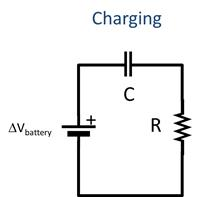
\includegraphics[width=1.67in,height=1.67in]{PH4CAW37}
	\caption{Charging and RC circuit.}
	\label{fig:rc_charge}
\end{figure}

Let's start by thinking of hooking up a capacitor and a resistor in series
with a battery, as seen in Figure \ref{fig:rc_charge}. 
The capacitor will become charged. The voltage across the
capacitor as a function of time will be given by

\begin{equation*}
\Delta V_{C}\left( t\right) =\Delta V_{\max }\left( 1-e^{-\frac{t}{\tau }%
}\right)% \qquad \text{charging}
\end{equation*}%
where 
\begin{equation}
\tau =RC
\end{equation}%
is the product of the resistance ($R$) and the capacitance ($C$), and 
is called the \emph{time constant}. The current
in the circuit as a function of time will be given by%
\begin{equation*}
I\left( t\right) =I_{\max }e^{-\frac{t}{\tau }}%\qquad \text{charging}
\end{equation*}%
while we charge up the capacitor. 

We should review what a time constant is. Think of a particular case, say, 
\begin{eqnarray*}
\Delta V_{battery} &=&1.5\unit{V} \\
R &=&2\unit{%
%TCIMACRO{\U{3a9}}%
%BeginExpansion
\Omega%
%EndExpansion
} \\
C &=&10\unit{F}
\end{eqnarray*}%
then%
\begin{equation*}
V_{C}(t)=\left( 1.5\unit{V}\right) \left( 1-e^{-\frac{t}{\left( 2\unit{%
%TCIMACRO{\U{3a9}}%
%BeginExpansion
\Omega%
%EndExpansion
}\right) \left( 10\unit{F}\right) }}\right)
\end{equation*}%
and 
\begin{eqnarray*}
\tau &=&\left( 2\unit{%
%TCIMACRO{\U{3a9}}%
%BeginExpansion
\Omega%
%EndExpansion
}\right) \left( 10\unit{F}\right) \\
&=&\allowbreak 20.0\unit{s}
\end{eqnarray*}%
We can plot the voltage as a function of time, as seen in 
Figure \ref{fig:rc_voltage}.
\begin{figure}[tbp!]
	\centering
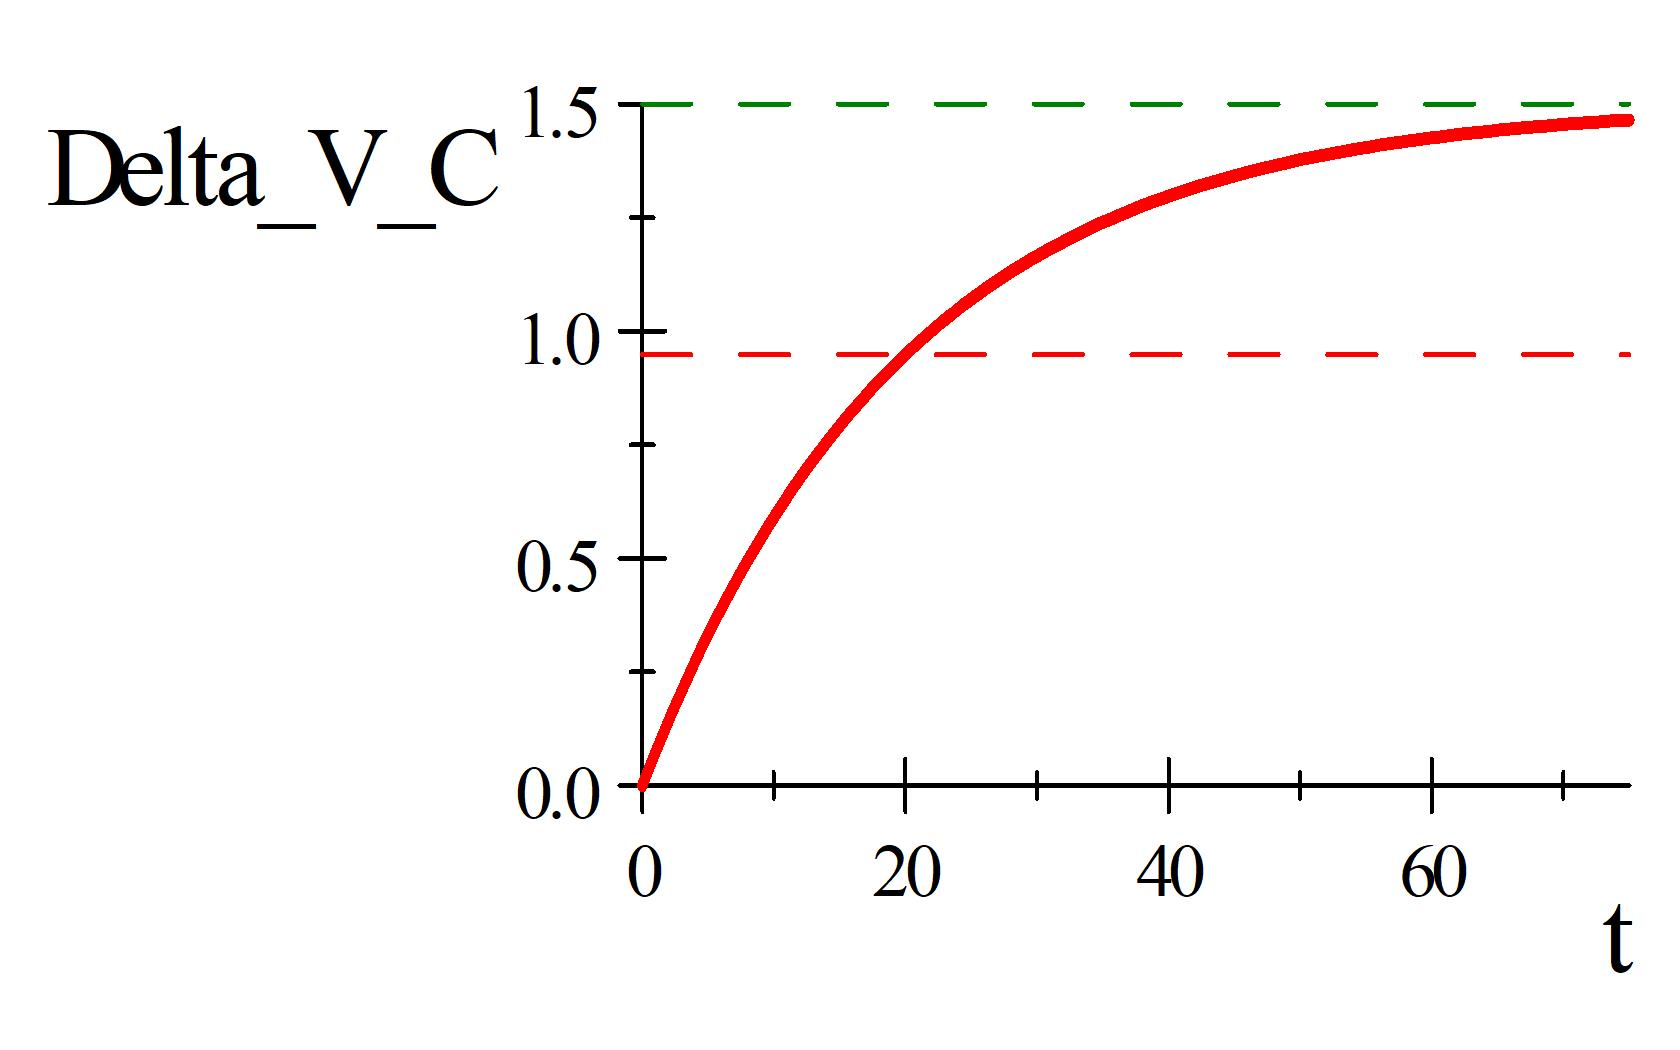
\includegraphics[width=2.8885in,height=1.58in]{PH4CAW38}
	\caption{The voltage in a charging RC circuit as a function of time.}
	\label{fig:rc_charge}
\end{figure}
Notice, that by about $t=70\unit{s%
}$ we essentially have $\Delta V_{C}=\Delta V_{battery}.$ But up to that
point, the voltage across the capacitor changes in a very non-linear way.
The part of the equation that looks like%
\begin{equation*}
\left( 1-e^{-\frac{t}{RC}}\right)
\end{equation*}%
is interesting. You should recall that $e^{0}=1$, so at $t=0$ we do have 
$\Delta V_{C}=0$ on the capacitor.
%because 
%\begin{equation*}
%\left( 1-e^{-\frac{t}{RC}}\right) =\left( 1-1\right)
%\end{equation*}%
For any positive time, $e^{-\frac{t}{RC}}$ will be less than $1.$ For large
positive times $\frac{t}{RC}$ gets to be a big number. So $e^{-\frac{t}{RC}}$
gets very small. Then $\left( 1-e^{-\frac{t}{RC}}\right) $ gets very close
to $1.$ That means that 
\begin{equation*}
\underset{t\rightarrow \infty }{\lim }\Delta V_{C}=\underset{t\rightarrow
\infty }{\lim }\Delta V_{battery}\left( 1-e^{-\frac{t}{RC}}\right) =\Delta
V_{battery}\left( 1\right) =\Delta V_{battery}
\end{equation*}%
just as we saw in the graph.

But what if $t=\tau =RC?$ Then 
\begin{eqnarray*}
\Delta V_{C} &=&\Delta V_{battery}\left( 1-e^{-\frac{RC}{RC}}\right) = \\
&=&\Delta V_{battery}\left( 1-e^{-1}\right) \\
&=&\allowbreak 0.632\,12\Delta V_{battery} \\
&\approx &63\%\Delta V_{battery}
\end{eqnarray*}%
The time $\tau $ is the time it takes for the capacitor to be $63\%$ charged!
The quantity $\tau $ is called the \emph{time constant} because it tells us
something about how long it takes for $\Delta V_{c}$ to go from $0$ to get
to $\Delta V_{battery}.$ 
%The \textquotedblleft
%t-looking-thing\textquotedblright\ is a Greek letter \textquotedblleft
%t.\textquotedblright\ It is pronounced \textquotedblleft
%tau.\textquotedblright\ This quantity will be useful in planning your
%experiment.

Notice what we have done. We have used our model to form an equation, and we
have used part of that equation to understand how much time it will take to
perform a test (experiment) of the model. This is typical, we have to get an
idea of how to make the measurement from the model we are testing.

%``But,'' you say, ``I don't really remember where all of these equations came
%from.'' Maybe your electricity and magnetism 
%class hasn't gotten to allowing current to flow
%yet so you have not done this. If any of this is mysterious, please read the
%section of our PH220 book that covers RC circuits. But if it is vaguely
%familiar or seems to make sense, really we can test our model of how
%capacitors work just knowing a little about capacitors and the equations
%that came from the model.

\section{The Instrument}

To test our capacitor model we need to measure the voltage across the
capacitor as a function of time. (We could also measure the current in the
circuit as a function of time, and either one of these is 
sufficient to test the model. For what follows, our focus will be on 
measuring the voltage. You know from a previous lab how we might add current
as a function of time.)

We've already seen how an Arduino can measure voltage and record it as a
function of time.
%We need a device that measures voltage and how it changes as a function of
%time. But that is just what our Arduino's do! We already know how to build
%this device. 
Suppose we can live with a $0\unit{V}$ to $+5\unit{V}$ range of 
$\Delta V_{battery}.$ Then even our simple voltmeter will work. Since it is
a function of time that we are testing, we need to output both voltage and
time from our Arduino. We can't guarantee that either of our capacitor leads
will be at ground, so we will have to be careful in wiring this voltmeter to
give $\Delta V_{C}.$

Remember that $\Delta V_{C}$ is the difference between two voltage
measurements. 
For our capacitor, the voltage difference can be found by 
\begin{equation*}
\Delta V_{C}=V_{2}-V_{1}
\end{equation*}%
where $V_2$ and $V_1$ are the potentials on either side of the capacitor
(see Figure \ref{fig:rc_wiring}),
neither of which will be ground. We really have to measure both with our
Arduino, and we also need a ground connection. The wiring diagram to do this
is seen in Figure \ref{fig:rc_wiring}. The sketch will be similar to one from
a previous lab.
\begin{figure}[htbp!]
	\centering
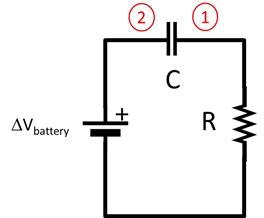
\includegraphics[width=0.3\textwidth]{PH4CAW39}
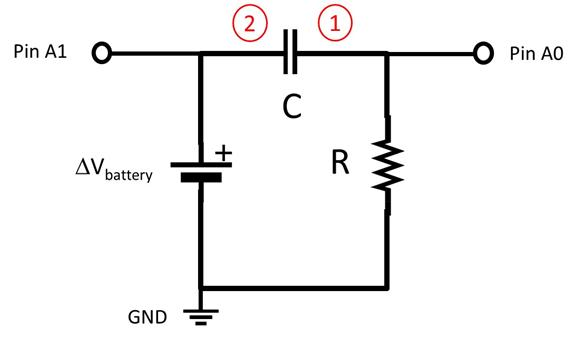
\includegraphics[width=0.5\textwidth]{PH4CAW3A}
	\caption[Wiring the RC circuit to the Arduino]{Wiring the RC circuit 
	to the Arduino. The left panel indicates the two voltages that we
	need to measure, and the right panel shows where we would connect
	the circuit to the Arduino pins.}
	\label{fig:rc_wiring}
\end{figure}

%\href{https://dtoliphant.github.io/PH250Manual/Code/RC_Volts_vsTime.ino}{Download here}
\lstinputlisting[language=Arduino]{Code/RC_Volts_vsTime.ino}

This sketch is similar to our simple voltmeter, except that it
uses two ADC pins and a ground. This
sketch also gives us time using the \code{millis()} function. 
This function gives
the number of milliseconds since our experiment began. We can use our python
code from a previous lab to save the data into a file. This code is 
similar to our previous version, with a few modifications.

%\href{https://dtoliphant.github.io/PH250Manual/Code/RC_ReadSaveFile.py}{Download here}
\inputpython{Code/RC_ReadSaveFile.py}{0}{10000}


\section{Fitting the Data}

\begin{figure}[htbp!]
	\centering
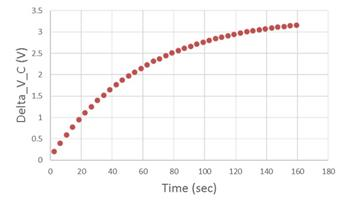
\includegraphics[width=2.9101in,height=1.7538in]{PH4CAX3B}
	\caption{Sample data for the RC circuit capacitor voltage.}
	\label{fig:rc_data}
\end{figure}
The data we collect with our instrument, when plotted, might look something 
like Figure \ref{fig:rc_data}.
You can make this plot in Excel, but 
Excel doesn't have the right function built into it for a
curve fit. We will use a different analysis program called LoggerPro. It is not
hard to use, and you can copy your data from a file (or from Excel) into
LoggerPro easily. The next section shows how to make this work. If you are a
fantastic Python programmer, you could use Python for this part. If you are
a die-hard Excel user, it is possible to use Excel and get the same
result (but not very easy). 

\subsection{LoggerPro Curve Fitting}

\begin{figure}[htbp!]
	\centering
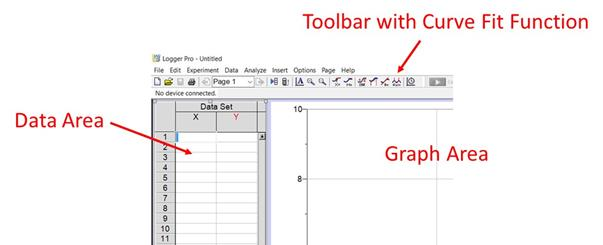
\includegraphics[width=5.0721in,height=2.0721in]{PH4CAX3D}
	\caption{The LoggerPro interface.}
	\label{fig:loggerpro}
\end{figure}
Let's start by noting that you can download LoggerPro to your own computer
if you would like. You should have received instructions for doing so from 
your instructor.
When you open LoggerPro, the window will appear similar to 
Figure \ref{fig:loggerpro}.
You will note that on the left side of the screen there is a spreadsheet-like
area that holds your data, and on the right is a graph of the data. The toolbar
at the top includes the functions we will need to fit our data.

If you have already imported your data into Excel or some other program, it
can be copied and pasted into the data area in LoggerPro. Place the time data
in the ``X'' column, and the voltage data in the ``Y'' column. When you have 
done so, LoggerPro will graph the data, and you will see something like 
Figure \ref{fig:rc_datagraph}.

%Suppose you have already imported your data in Excel. It might look
%like this:
%\begin{figure}[h!]
%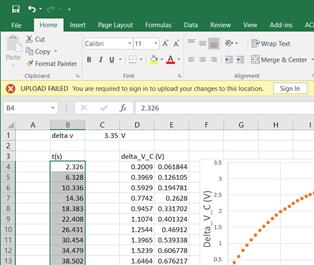
\includegraphics[width=2.6498in,height=2.2399in]{PH4CAX3C}
%\end{figure}
%Now highlight a----- column (I
%%highlighted the time column) and select copy to copy the data to the
%clipboard. Then open up LoggerPro. You will see a data area, a graph area,
%and the toolbar.
%We want to past the data into a
%column in LoggerPro. If you also selected the time data, paste it into the $%
%x $-column in Logger Pro. 
%\begin{figure}[h!]
%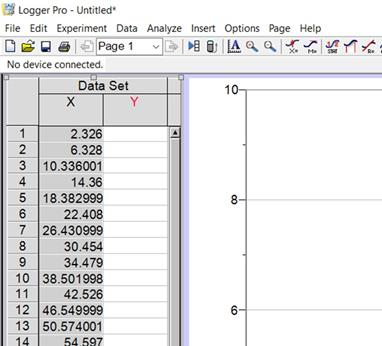
\includegraphics[width=3.2197in,height=2.9187in]{PH4CAX3E}
%\end{figure}

%Do the same for the voltage data. Paste it into the $y$-column. Once you do
%this, the data will automatically be graphed. 
\begin{figure}[htbp!]
	\centering
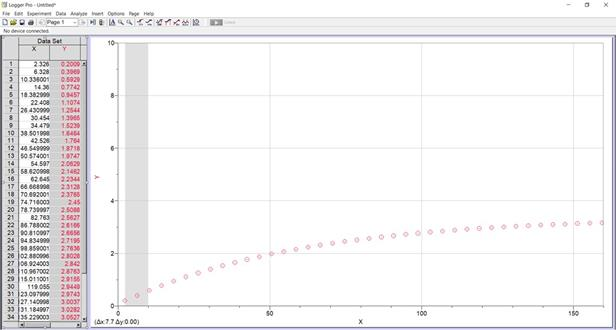
\includegraphics[width=0.8\textwidth]{PH4CAX3F}
	\caption{Capacitor voltage graphed in LoggerPro.}
	\label{fig:rc_datagraph}
\end{figure}

We now want to fit a curve to
this data. The curve fit function can be accessed from the tool bar. The button
is shown in the left panel of Figure \ref{fig:curvefit}. When you click this
button, a dialog box will appear. This dialog box can be seen in the right
panel of Figure \ref{fig:curvefit}.

\begin{figure}[htbp!]
	\centering
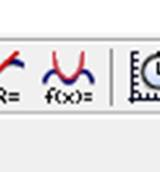
\includegraphics[width=0.15\textwidth]{PH4CAX3G}
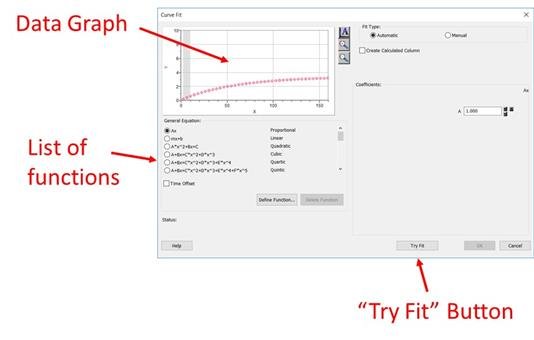
\includegraphics[width=0.75\textwidth]{PH4CAX3H}
	\caption{The curve fit button and dialog in LoggerPro.}
	\label{fig:curvefit}
\end{figure}

It may be tempting to try just any function to see if it fits. 
Remember, though, that our goal is
not to have a great fit. The goal is to see if our data fit the equation
from our capacitor model. 
\begin{equation*}
\Delta V_{C}\left( t\right) =\Delta V_{\max }\left( 1-e^{-\frac{t}{\tau }%
}\right)
\end{equation*}%
We need to find this particular function (which is not one of the default
functions in Excel).
\begin{figure}[tbp!]
	\centering
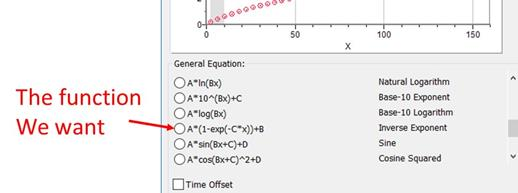
\includegraphics[width=3.2759in,height=1.2298in]{PH4CAX3I}
	\caption{The LoggerPro fit function needed for our model.}
	\label{fig:fitfunction}
\end{figure}
Of course, we won't find a match
with our exact notation. The one we want is given as 
\begin{equation*}
y=A\ast (1-\exp (-C\ast x))+B
\end{equation*}%
in LoggerPro (Figure \ref{fig:fitfunction}), 
and now we have to match our variables with theirs. 
Let's compare the
equations. 
\begin{eqnarray*}
y &=&A\ast (1-\exp (-C\ast x))+B \\
\Delta V_{C}\left( t\right) &=&\Delta V_{\max }\left( 1-e^{-\frac{t}{\tau }%
}\right) +0
\end{eqnarray*}%
We can see that our $\Delta V_{\max }$ corresponds to their $A$, and our 
$\tau$ corresponds to their $1/C$. Our equation doesn't have a variable
corresponding to their $B$.

Knowing what the variables will represent for our equation, we can now see
how well the function fits our data. Do this by clicking the ``Try Fit'' button
in the lower right portion of the dialog. 
%(Figure \ref{fig:tryfit}).
%\begin{figure}[htbp!]
%	\centering
%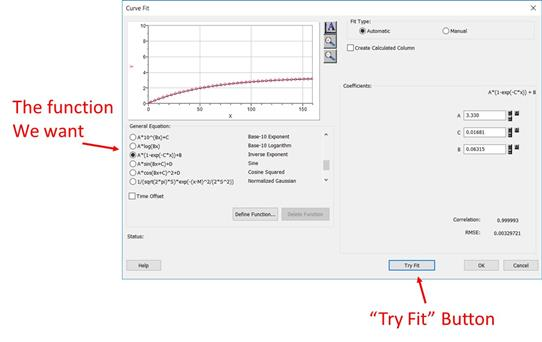
\includegraphics[width=4.561in,height=2.8842in]{PH4CAX3J}
%	\caption{Location of the ``Try Fit'' button.}
%	\label{fig:tryfit}
%\end{figure}

If the fit looks good, choose the \textquotedblleft OK\textquotedblright\
button. You will return to the main LoggerPro window, and will see your
graph, but now with the line of best fit and a new little box
(Figure \ref{fig:fitcomplete}). 
\begin{figure}[tbp!]
	\centering
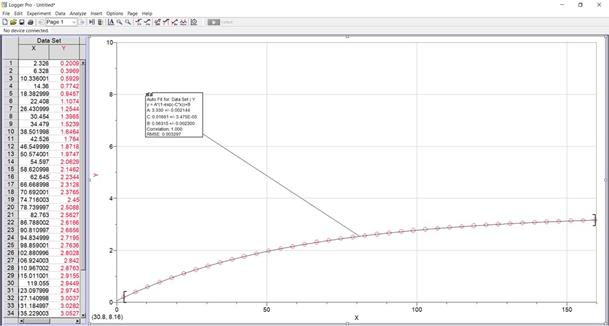
\includegraphics[width=0.6\textwidth]{PH4CAX3K}
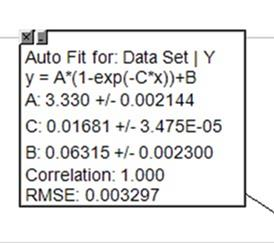
\includegraphics[width=0.3\textwidth]{PH4CAX3L}
	\caption[The LoggerPro window after completing the fit]{The LoggerPro
	window after completing the fit. The left panel shows the main window,
	and the right panel shows the detail of the box containing the fit
	parameters.}
	\label{fig:fitcomplete}
\end{figure}
The curve fit looks nice and that
is comforting. For the data shown here, 
it looks like our capacitor model might be
correct, but we can't be sure until we add in error bars. Before we do that,
though,
let's look at the new little box (Figure \ref{fig:fitcomplete}, right panel). 
The box has our fit equation that
we chose, and it has values for the fit parameters and their uncertainties.
We will need those later!

Let's add on the error bars now. Right click on the graph if you have a PC
or do the Mac equivalent if you have a Mac. A new dialog appears and in this
case choose \textquotedblleft Graph Options\textquotedblright\ 
(Figure \ref{fig:graphopts}, left panel).
\begin{figure}[tbp!]
	\centering
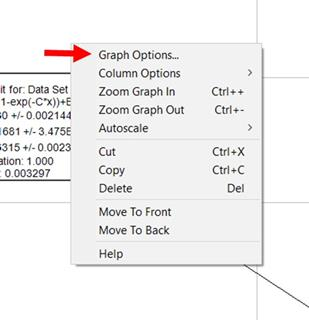
\includegraphics[width=0.3\textwidth]{PH4CAX3M}
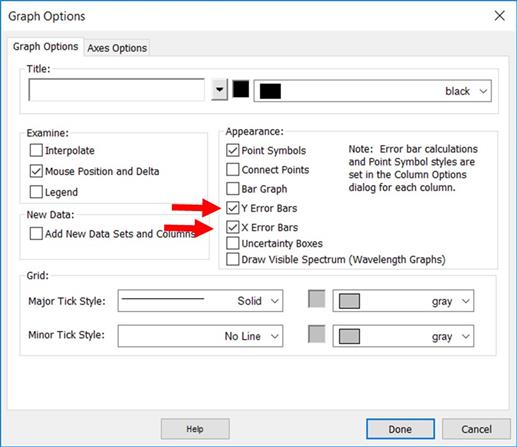
\includegraphics[width=0.5\textwidth]{PH4CAX3N}
	\caption[LoggerPro graph options]{LoggerPro graph options, used to
	add error bars to the graph. The left panel shows the pop up menu
	that appears upon right clicking the graph. The right panel shows the
	graph options dialog.}
	\label{fig:graphopts}
\end{figure}%
On the \textquotedblleft Graph Options\textquotedblright\ dialog make sure
both $x$ and $y$-error bars are checked.
Chose \textquotedblleft
Done\textquotedblright. 

Right click on the graph again. This time choose
\textquotedblleft Column Options\textquotedblright\ 
(Figure \ref{fig:colopts}, left panel).
\begin{figure}[tbp!]
	\centering
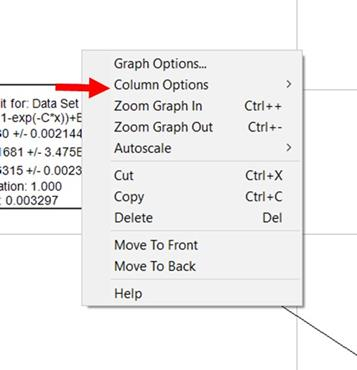
\includegraphics[width=0.3\textwidth]{PH4CAX3O}
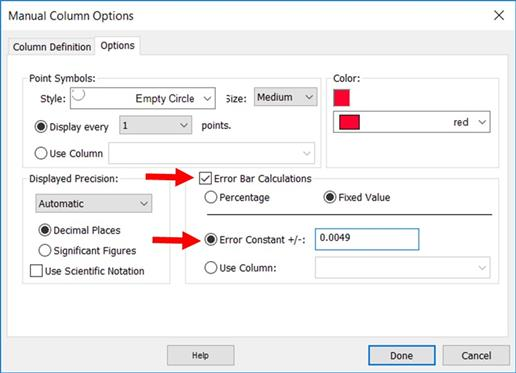
\includegraphics[width=0.5\textwidth]{PH4CAX3P}
	\caption[LoggerPro column options]{LoggerPro column options. The left
	panel shows the pop up menu that appears upon right clicking the 
	graph. The right panel shows the dialog for the $y$ data set.}
	\label{fig:colopts}
\end{figure}
In the dialog, choose the $y$-data set.
Another dialog appears with two tabs
(Figure \ref{fig:colopts}, right panel). Choose the \textquotedblleft
Options\textquotedblright\ tab. 
You will see a place to choose how error bars are calculated. If you used
the simple voltmeter sketch as your basis, you know the quantization error
is about $4.9\unit{mV}.$ That will be true for every voltage measurement so
we can input this as a constant value. If you used a voltage divider, you
will have to use your calculated error value here. When you have your error
value in place, choose \textquotedblleft Done\textquotedblright. The final
product will look like Figure \ref{fig:rc_done}.
\begin{figure}[htbp!]
	\centering
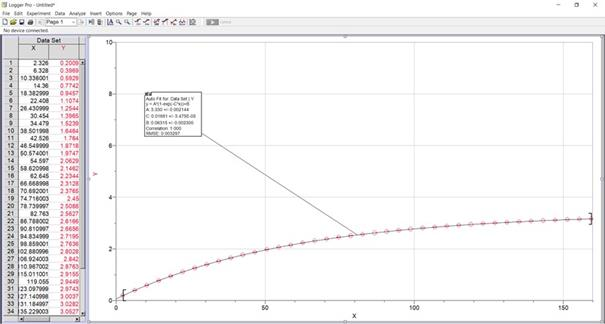
\includegraphics[width=5.0886in,height=2.7345in]{PH4CAX3Q}
	\caption{The final graph, now with error bars.}
	\label{fig:rc_done}
\end{figure}

The voltage error was so small that it is hard to see the error bars! That
is fine. What this tells us is that our fit line must go right through the
center of each data point, so we are really doing fine. The
data supports the model.

But now let's go back to our little box of curve fit parameters. We
identified 
\begin{equation*}
\tau =\frac{1}{\mathtt{C}}
\end{equation*}%
and for my data I have 
\begin{equation*}
\mathtt{C}=0.01681\pm 3.475\times 10^{-5}
\end{equation*}%
\newline
We need units, and looking at the equation we know $\tau $ has units of
seconds, so $\mathtt{C}$ must have units of inverse seconds.%
\begin{equation*}
\mathtt{C}=\left( 0.01681\pm 3.475\times 10^{-5}\right) \frac{1}{\unit{s}}
\end{equation*}%
so we can find a value for $\tau .$ For my data, I have 
\begin{eqnarray*}
\tau _{measured} &=&\frac{1}{0.01681\frac{1}{\unit{s}}} \\
&=&59.\,\allowbreak 488\unit{s}
\end{eqnarray*}

Note that we will have to calculate the uncertainty in $\tau .$ I will leave
that for an exercise. But I can compare this $\tau _{measured}$ to the $\tau
=RC$ value I started with. If they are within each other's error range, this
is a powerful confirmation of our capacitor model.

\activity
{
We have two equations that describe the voltage across the capacitor and
the current in an RC circuit as a function of time:
\begin{eqnarray*}
	\Delta V_{C}\left( t\right) &=&\Delta V_{\max }\left( 1-e^{-\frac{t}{\tau }%
}\right) \\
	I\left( t\right) &=&I_{\max }e^{-\frac{t}{\tau }}
\end{eqnarray*}%
where $\tau =RC$
is the time constant. As you complete these activities, follow good lab
notebook procedures by recording everything!

\begin{enumerate}
\item Using a capacitor with a capacitance of about 20 $\mu$F
and a resistor of about 1 M$\Omega$,
create a series RC circuit. You can power your circuit with a power supply,
but be careful to stay in the $0\unit{V}$ to $+5\unit{V}$
range (or to use a voltage divider to achieve this range at the Arduino
input). Note that we will be using electrolytic capacitors today, which only
work in one direction. If the circuit doesn't work, try turning your capacitor
around.

\item Predict the time constant for your circuit, using the resistance and
	capacitance values.
\item Build your instrument, write the sketch, and write the Python collection
code. Test every part of the instrument before you start collecting
capacitor data. Don't forget to find your uncertainties. 

\item Work with a lab
partner from your group and collect the voltage data for your charging
capacitor. Compare your data
among your group to make sure things went well. Record your data in your
lab notebook, or give a location of where the data is stored.

\item Graph your data. LoggerPro is fine for both
graphing and the curve fit (next item). You should include this graph in
your lab notebook (but might also include the curve fit described in the
next item on the same graph).

\item Perform the curve fit. As in the last lab, having the proper curve fit
the data is a validation of our model! So if the thoretical curve fits the
data, it makes sense that something about the model is right. Include the
graph of the curve fit and the data in your lab notebook as well as the fit
equation and fit parameters (don't forget their uncertainties).

\item Find the time constant from your fit, and compare to your 
	predicted value. If these
compare within their uncertainties, we have a further validation of the
model. Record the time constants and their uncertainties in your lab
notebook.

\item Draw a conclusion: is our capacitor model good?
\end{enumerate}
}
